\documentclass[a4paper,12pt,twoside]{ThesisStyle}
\usepackage[utf8]{inputenc}
\usepackage[english]{babel}
\usepackage{thesis-style}
\usepackage{wrapfig}
\usepackage{graphicx}
\usepackage{hyperref}


\begin{document}

\frontmatter

\pagenumbering{gobble}

\thispagestyle{empty}
\begin{table}[htb]
\centering
\begin{Large}
\resizebox{\textwidth}{!}{\begin{tabular}{ | l |}
 \hline
 \\

\includegraphics[scale=0.9]{imatges/logo_eps.png} \\[0.7cm]
\centerline{Treball Final de Màster}\\[1cm]
\hline
\\
Study: Master in Data Science and Machine Learning\\[0.7cm]
\hline
\\
Title: CNV Detection using Machine Learning in Targeted Sequencing\\[0.7cm]
\hline
\\
Document: Memory\\[0.7cm]
\hline
\\
Student: Oriol Canal Pujol\\[0.7cm]
\hline
\\
Tutor: Maria Beatriz Lopez Ibañez\\
Department: Grup de Recerca en Enginyeria de Control i Sistemes Intel·ligents (EXIT)\\
Àrea: ENGINYERIA DE SISTEMES I AUTOMÀTICA\\
Cotutor: Bernat del Olmo Cabestré \\[0.7cm]
\hline
\\
Call: September 2024\\[0.7cm]
\hline

\end{tabular}}
\end{Large}
\end{table}

\newpage
\hypersetup{pageanchor=false}
\begin{titlepage}

% Upper part of the page

\includegraphics[scale=0.9]{imatges/logo_eps.png} \\[1cm]
\begin{center}
\textsc{\Large Master Thesis} \\[1cm]

% Title
\begin{spacing}{2}
\HRule \\
\textbf{\Huge CNV Detection using Machine Learning in Targeted Sequencing} \\
\HRule \\[0.5cm]
\end{spacing}

% Author and supervisor and other data
{
\large
\emph{Author:} \\
Oriol \textsc{Canal Pujol} \\[1cm]
September 2024 \\[1cm]
Master in Data Science and Machine Learning \\[1cm]
\emph{Tutors:} \\
Beatriz \textsc{Lopez Ibañez} \\
Bernat \textsc{del Olmo Cabestré} \\
}

\end{center}
\end{titlepage}
\hypersetup{pageanchor=true}

\titlepage

%\dominitoc


\pagenumbering{roman}

\chapter*{Resum}
%\label{cap:resum}



\chapter*{Agraïments}
%\label{cap:agraiments}

Per començar vull agrair molt especialment a \ldots


\tableofcontents

\listoffigures

\listoftables

\mainmatter

\chapter{Introduction}
\label{cap:intro}
\section{Next Generation Sequencing}
In recent years, advancements in technology have significantly enhanced our ability to study the genetic material of living organisms. One of the most groundbreaking developments in this field is Next Generation Sequencing (NGS). NGS is a transformative genomic sequencing technology that enables researchers and clinicians to rapidly and cost-effectively analyze vast amounts of genetic data. This advanced method facilitates the identification of disease-causing pathogens and cancer-associated mutations in patient genomes with enhanced speed and precision. By significantly reducing the time and cost associated with genetic analysis, NGS has revolutionized the fields of genomics and personalized medicine, providing critical insights into the genetic underpinnings of various diseases.

NGS technology represents a significant advancement over traditional sequencing methods, such as Sanger sequencing, by allowing for high-throughput sequencing that can cover entire genomes or specific genomic regions of interest. This high-throughput capability is particularly beneficial for comprehensive studies of genetic variation. Single Nucleotide Polymorphisms (SNPs), which are single nucleotide differences in the DNA sequence, and insertions and deletions (indels), small additions or losses of DNA bases, are common types of genetic variations detected through NGS. SNPs occur frequently and contribute to genetic diversity among individuals, while indels can affect gene function depending on their location within the genome.

Another important type of genetic variation detected by NGS is Copy Number Variants (CNVs), which involve duplications or deletions of large genomic segments. CNVs can range in size from thousands to millions of base pairs and are known to influence gene dosage and expression levels. These structural variations are implicated in various diseases, including developmental disorders and cancers, making them crucial targets for genetic research and clinical diagnostics.

The ability to sequence multiple samples simultaneously with high accuracy makes NGS a powerful tool in both research and clinical settings. It enables comprehensive studies of genetic variation across populations and facilitates the identification of disease-causing mutations with unprecedented speed and precision. As NGS technology continues to evolve, its impact on genomics and personalized medicine is expected to grow, further enhancing our understanding of genetic mechanisms underlying health and disease.

\subsection{Targeted Sequencing}

Targeted sequencing is a specialized approach in genomic analysis that enables researchers to selectively sequence specific regions of interest within the genome. Unlike whole-genome sequencing, which sequences the entire genome indiscriminately, targeted sequencing focuses on predefined genomic regions. This method is particularly advantageous in studies where a comprehensive analysis of the entire genome is unnecessary or cost-prohibitive.
\begin{figure}[htb]
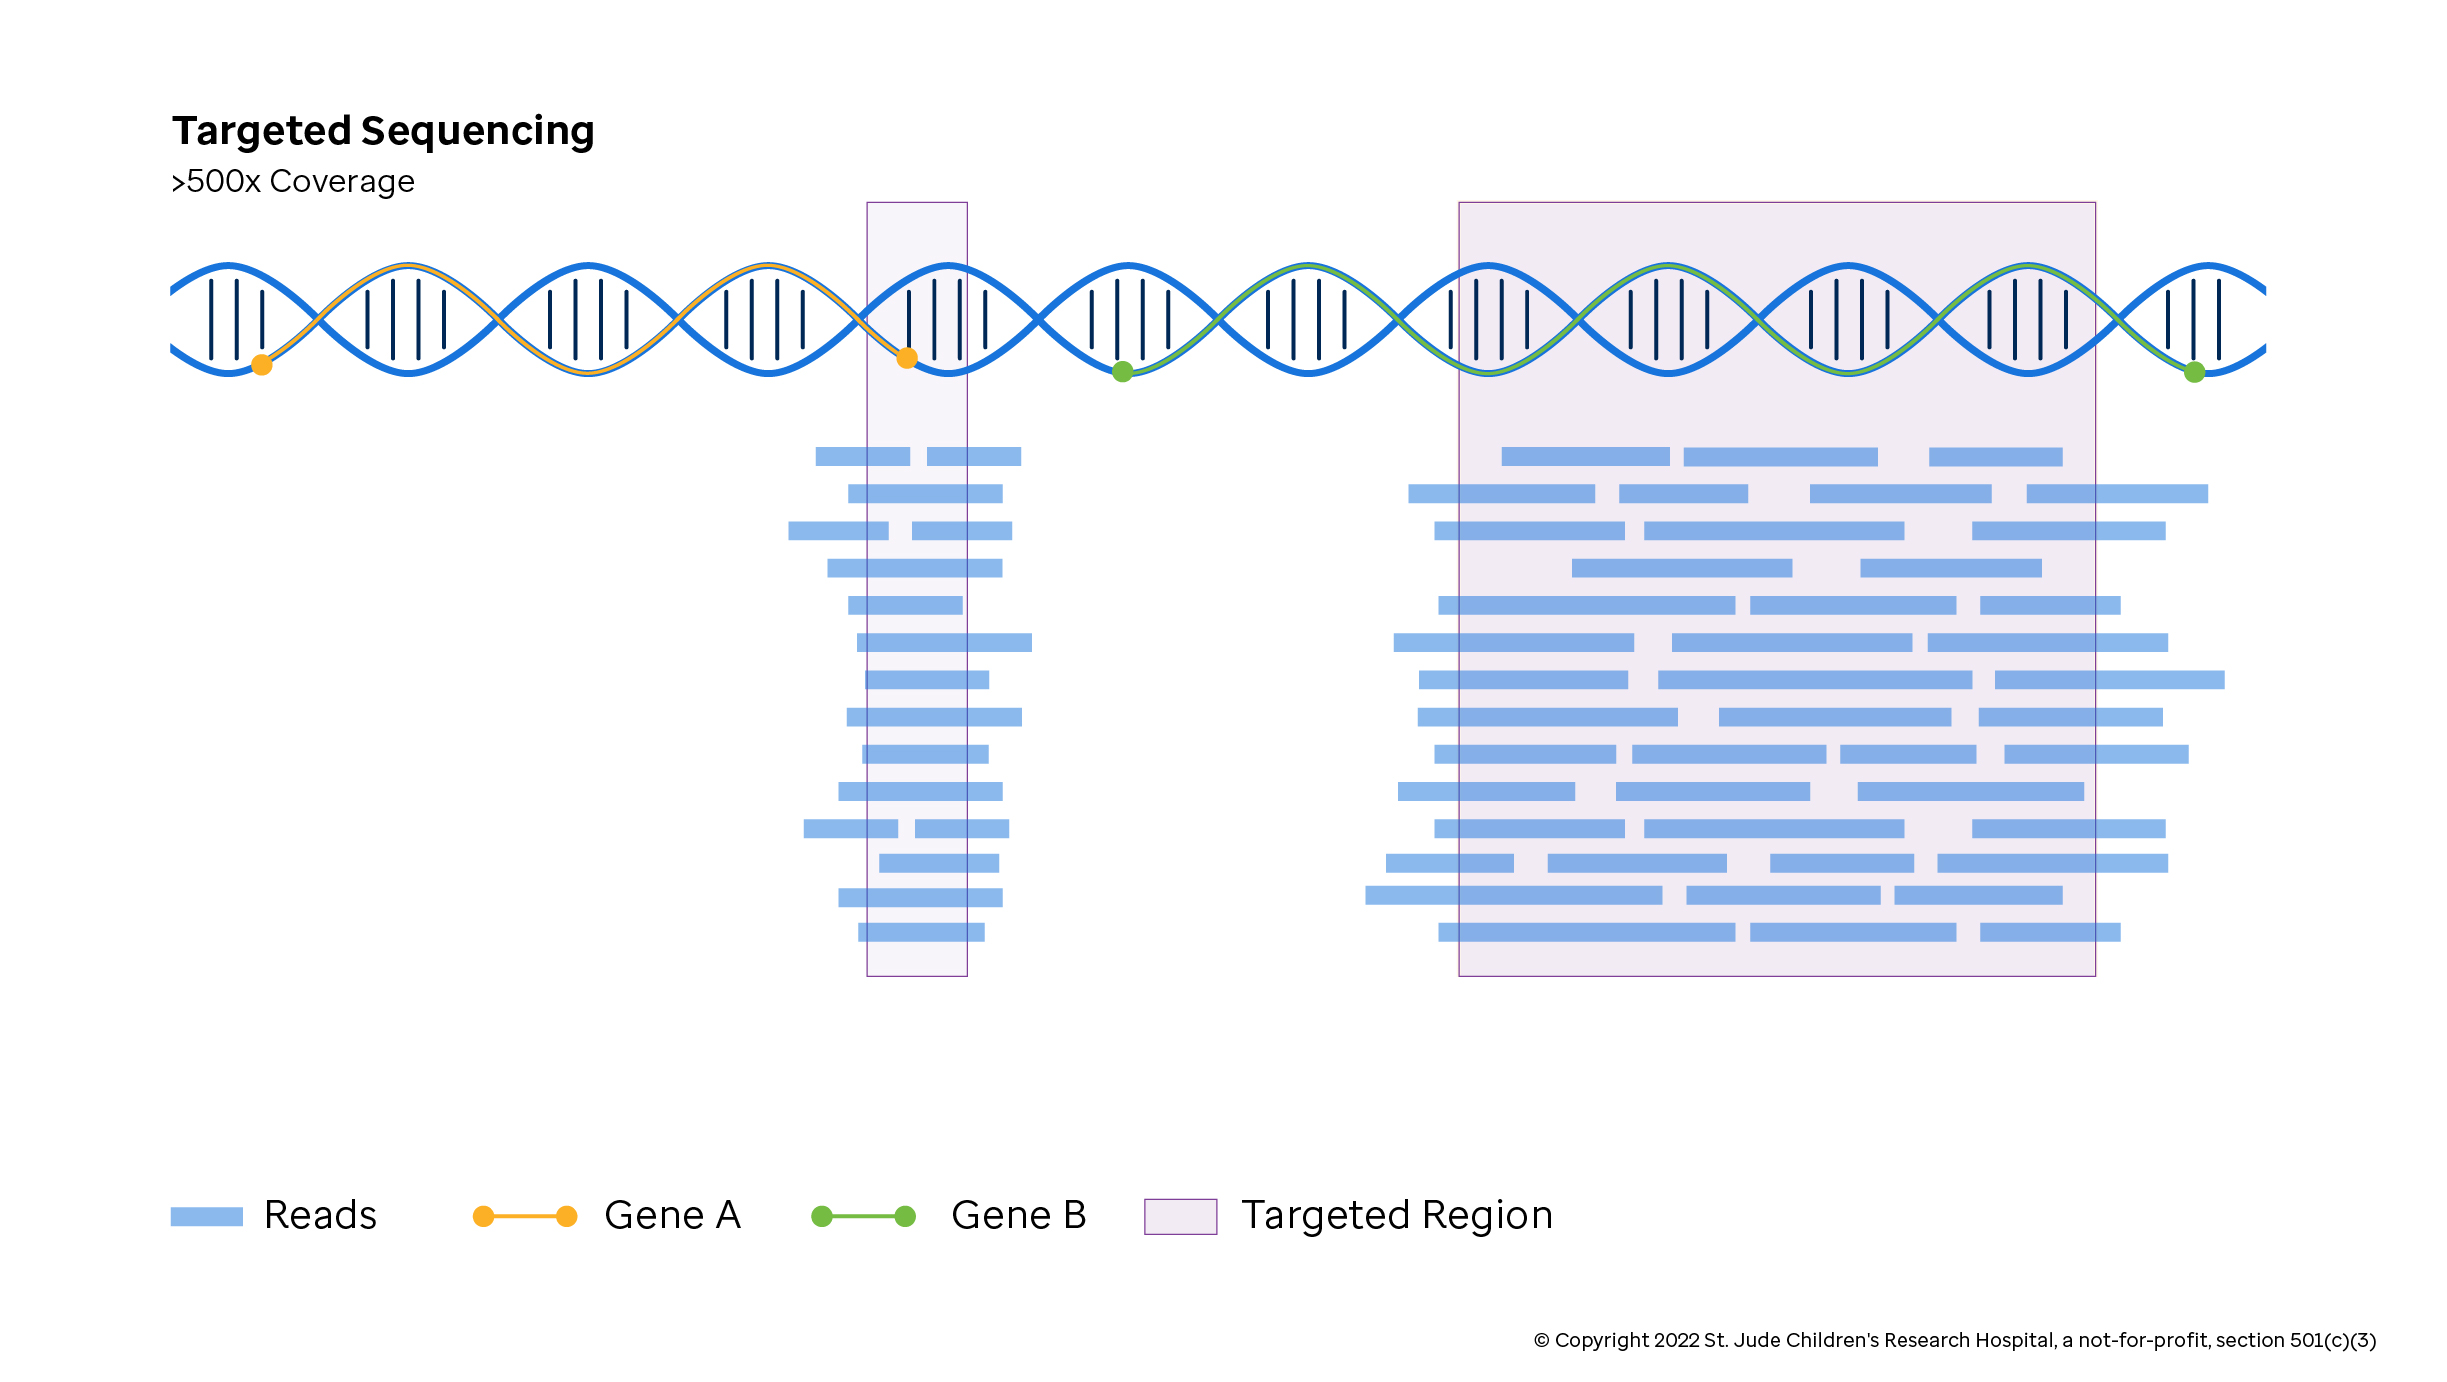
\includegraphics[width=15 cm]{imatges/targeted_sequencing.jpg}
\caption{\label{fig:logo} Illustrates the comprehensive workflow of genomic DNA targeted sequencing.}
\end{figure}
Targeted sequencing involves several key steps:

\begin{itemize}
    \item \textbf{Genomic DNA Library Preparation}: The initial step in targeted sequencing is the preparation of a genomic DNA library. This involves extracting genomic DNA from a sample, such as blood or tissue, and fragmenting it into smaller pieces using mechanical or enzymatic methods. The fragmented DNA ends are then modified to ensure they are ready for sequencing, and short synthetic sequences called adapters are attached to both ends of each fragment. In some cases, the library is amplified using polymerase chain reaction (PCR) to increase the quantity of DNA fragments.
    
    \item \textbf{Targeted DNA Enrichment}: Once the DNA library is prepared, the next step is to enrich for the regions of interest. This is achieved through hybridization capture, where probes—short, single-stranded DNA or RNA molecules that are complementary to the target regions—are used. These probes bind to their complementary sequences within the DNA library. The probe-bound DNA fragments are then captured using magnetic beads or another separation method, while non-target sequences are washed away. Finally, the target DNA fragments are released from the beads, resulting in an enriched library that predominantly contains the regions of interest.

    \item \textbf{Paired-End Sequencing}: The enriched DNA library is then subjected to paired-end sequencing, which involves sequencing both ends of each DNA fragment using a sequencing platform, such as Illumina. This platform reads the nucleotide sequence from each end of the DNA fragment, creating two reads per fragment. This paired-end approach improves the accuracy of alignment and variant detection.
    
    \item \textbf{Alignment to the Human Reference Genome}: The sequencing reads are mapped to a reference genome, such as GRCh38, to determine their origin within the genome. Bioinformatics tools like BWA or Bowtie align the paired-end reads to the reference genome, and the alignment information is stored in SAM (Sequence Alignment/Map) or BAM (Binary Alignment/Map) files, indicating the position of each read in the reference genome.
    
    \item \textbf{Variant Detection and Annotation}: Finally, the aligned reads are analyzed to identify genetic variants, which are differences between the sequenced sample and the reference genome. Bioinformatics tools such as GATK or FreeBayes detect single nucleotide polymorphisms (SNPs), insertions, deletions (indels), and copy number variants (CNVs). Quality filters are applied to remove low-confidence variants, and annotation tools like ANNOVAR, SnpEff or Variant Effect Predictor provide information on the genomic context and potential significance of the variants.

\end{itemize}
By following these steps, targeted sequencing provides a focused and efficient method for analyzing specific genomic regions, facilitating the identification of genetic variations associated with diseases and advancing our understanding of genetic underpinnings in various biological processes.
\begin{figure}[htb]
\centering
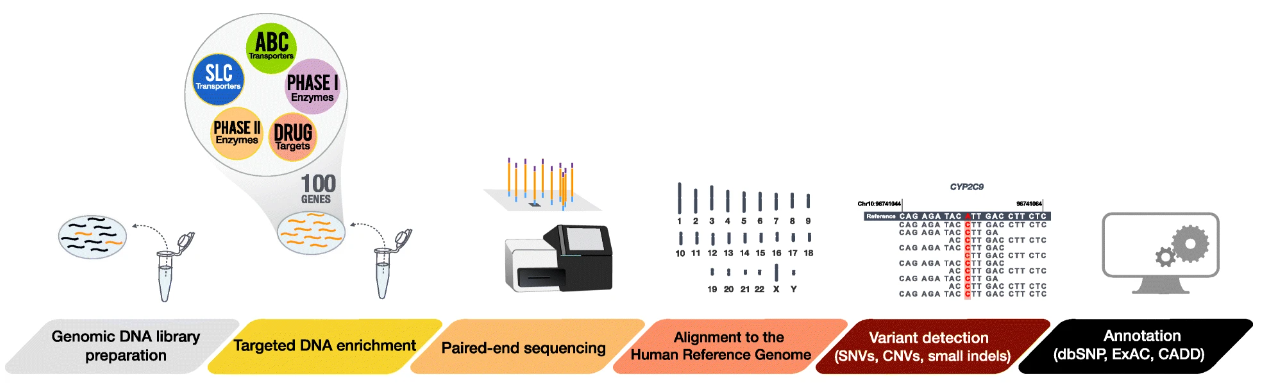
\includegraphics[width=15 cm]{imatges/DNA_sequencing.png}
\caption{\label{fig:logo} Illustrates the comprehensive workflow of genomic DNA targeted sequencing.}
\end{figure}

\section{COPY NUMBER VARIATIONS}

\begin{wrapfigure}{r}{0.5\textwidth} % 'r' for right, '0.5\textwidth' for the width of the figure environment
    \centering
    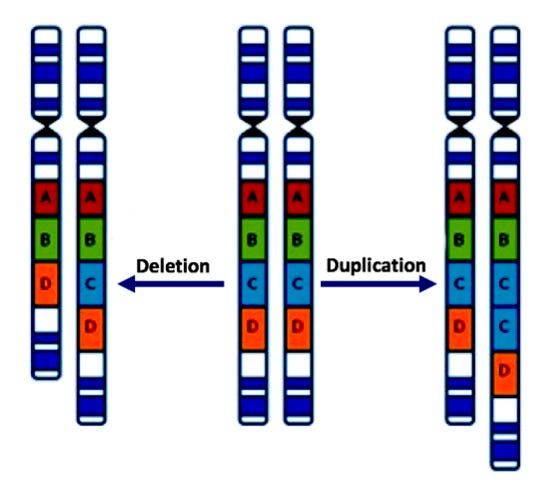
\includegraphics[width=0.48\textwidth]{imatges/CNV.jpg} % Adjust the width as necessary
    \caption{\label{fig:CNV} Illustrates the comprehensive workflow of genomic DNA targeted sequencing.}
\end{wrapfigure}

Copy Number Variations (CNVs) are a form of structural genetic variation characterized by the duplication or deletion of large segments of DNA, ranging from thousands to millions of base pairs (Figure~\ref{fig:CNV}). These variations can significantly impact gene dosage and expression levels, influencing phenotypic diversity and contributing to various disease processes. CNVs are particularly notable for their role in complex diseases, such as neurodevelopmental disorders, psychiatric conditions, radiological disorders and various cancers.
\\\\\\
CNVs can affect the patients in several ways:
\begin{itemize}

    \item \textbf{Gene dosage}: Changes in the number of gene copies can lead to overexpression or underexpression of genes, affecting cellular function and potentially leading to disease. For instance, duplications of oncogenes can drive cancer progression, while deletions of tumor suppressor genes can remove critical regulatory mechanisms that prevent uncontrolled cell growth.
    \item \textbf{Gene disruption}: CNVs can interrupt the coding sequence of genes, potentially leading to truncated or nonfunctional proteins. This can result in loss-of-function effects that disrupt normal biological processes.
    \item \textbf{Regulatory elements}: CNVs can encompass regulatory regions such as promoters or enhancers, altering gene expression patterns and contributing to phenotypic variation and disease susceptibility.
\end{itemize}

% \begin{figure}[htb]
% \centering
% 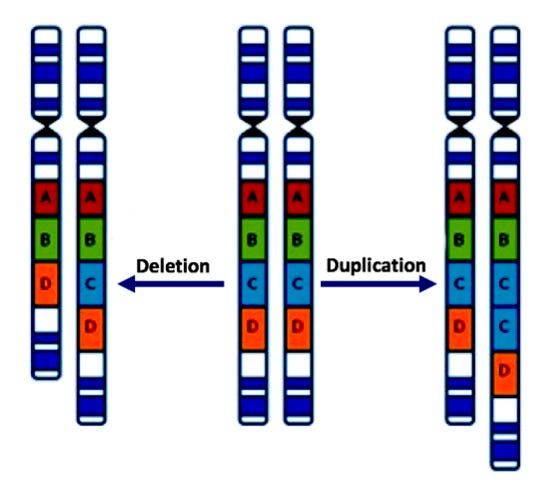
\includegraphics[width=8 cm]{imatges/CNV.jpg}
% \caption{\label{fig:logo} Deletion and duplication of the chromosomal region  C}
% \end{figure}
\subsection{Detection of CNVs}
Next-generation sequencing (NGS) is an outstanding technology for detecting single-nucleotide variants and small deletions and insertions in genetic testing for Mendelian conditions. However, detecting large rearrangements, such as copy-number variants (CNVs), from NGS data remains challenging due to issues intrinsic to the technology, including short read lengths and GC-content bias. Despite these challenges, it is well recognized that germline CNVs are the genetic cause of several hereditary diseases, making their analysis a necessary step in a comprehensive genetic diagnostics strategy.

Traditionally, the gold standards for CNV detection in genetic diagnostics have been multiplex ligation-dependent probe amplification (MLPA) and array comparative genomic hybridization (aCGH). While both methods are highly reliable, they are also time-consuming and costly, often leading to the testing of only a subset of genes and excluding others from the analysis, particularly in single-gene approaches. Thus, the ability to use NGS data as a first screening step for CNVs would significantly decrease the number of MLPA/aCGH tests required and conserve valuable resources.

\subsubsection{Challanges in detecting CNVs in targeted sequencing}
Numerous tools have been developed for CNV detection from NGS data. Most of these tools were originally designed for whole-genome or whole-exome sequencing and often struggle with the sparser data generated from targeted NGS panels used in routine genetic testing. Despite these challenges, several algorithms have been specifically adapted or developed to detect CNVs in targeted sequencing. Notable among these are DECON, GATK gCNV, and CNVKit. Each of these algorithms employs distinct strategies to analyze read depth, normalize data, and identify CNVs, contributing to their effectiveness in various research and clinical applications.

Detecting CNVs in targeted sequencing remains a difficult task due to several intrinsic challenges. The first major challenge is the inherent variability in read depth, which can be influenced by factors such as target capture efficiency, sequencing depth, and GC content. Variations in read depth can lead to both false positives and false negatives in CNV detection, making it crucial to apply robust normalization techniques to correct for these biases.

Another challenge is the short read lengths characteristic of NGS data, which can complicate the accurate alignment of reads to the reference genome, particularly in repetitive regions or regions with complex structural variations. Misalignment can lead to erroneous CNV calls, necessitating the use of sophisticated alignment algorithms and quality control measures to ensure accurate mapping.

Additionally, the targeted nature of sequencing panels means that only specific regions of the genome are sequenced, resulting in sparser data compared to whole-genome or whole-exome sequencing. This sparsity can make it difficult to accurately detect CNVs, especially those that span large genomic regions or occur in low-complexity regions. The reliance on targeted panels also means that any biases in probe design or capture efficiency can disproportionately affect the accuracy of CNV detection in certain regions.

\section{STATE OF THE ART}

The detection of CNVs in targeted sequencing has seen substantial advancements due to improvements in sequencing technologies and bioinformatics tools. 

Algorithms for CNV detection in targeted sequencing typically leverage read depth information, which reflects the number of sequencing reads mapping to specific genomic regions. Variations in read depth can indicate the presence of CNVs, but accurately detecting these variations requires overcoming technical biases, such as GC-content bias, sequencing depth variability, and capture efficiency inconsistencies.

Three prominent algorithms used for CNV detection in targeted sequencing are DECON, GATK gCNV, and CNVKit. These tools are designed to handle the nuances of targeted sequencing data, employing advanced statistical models and normalization techniques to distinguish true CNVs from background noise. Each algorithm has its unique approach to read depth analysis, normalization, and segmentation, contributing to their effectiveness in both research and clinical applications.
\begin{itemize}

    \item \textbf{GATK gCNV}: \href{https://github.com/broadinstitute/gatk}{The Genome Analysis Toolkit (GATK)} is a comprehensive suite of tools designed to facilitate the discovery of genetic variants from high-throughput sequencing data. Developed by the Broad Institute, GATK is widely recognized for its robustness, accuracy, and efficiency in processing and analyzing genomic data. GATK gCNV (germline Copy Number Variants) is a specialized component within the GATK toolkit designed to detect CNVs in germline genomes. GATK-gCNV pipeline (Figure~\ref{fig:gatk-gcnv}) begins by collecting coverage information from genome-aligned reads over a set of predefined genomic intervals (a). Next, the original interval list is filtered to remove coverage outliers, unmappable genomic sequence, and regions of segmental duplications (b). Then, samples are clustered into batches based on read-depth profile similarity using PCA and each batch is processed separately (c).  Chromosomal ploidies are inferred using total read-depth of each chromosome (d). Finally, The GATK-gCNV model learns read-depth bias and noise
and iteratively updates copy number state posterior probabilities until a selfconsistent state is obtained; after convergence, constant copy number segments are found using the Viterbi algorithm along with segmentation quality scores.
    \end{itemize}
    \begin{figure}[htb]
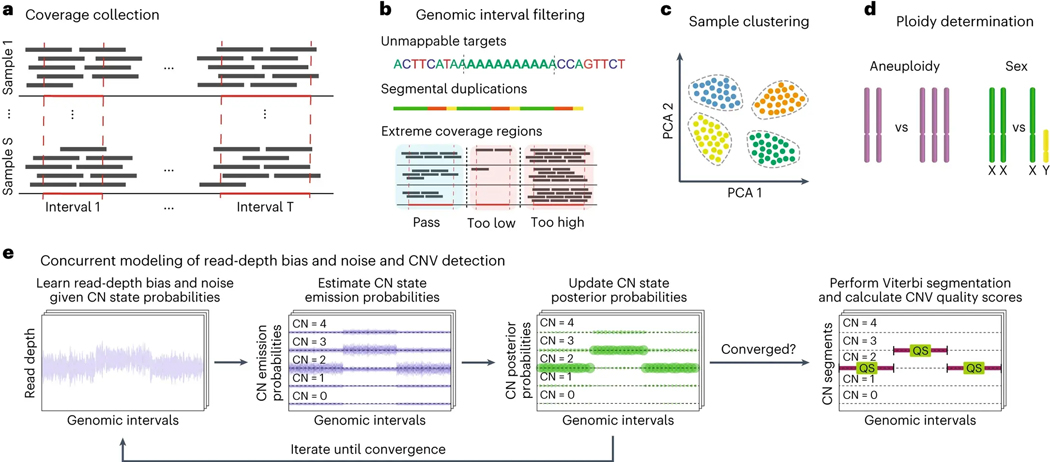
\includegraphics[width=13 cm]{imatges/gatk-gcnv.jpg}
\caption{\label{fig:gatk-gcnv} GATK-gCNV pipeline steps.}
\end{figure}
\begin{itemize}

    \item \textbf{DECoN}: \href{https://github.com/RahmanTeam/DECoN}{Detection of Exon Copy Number Variants (DECoN)} is a specialized algorithm designed to detect CNVs in exon regions using targeted sequencing data. To distinguish true CNVs from random fluctuations in read counts, DECoN employs a Bayesian statistical framework. This approach models the expected distribution of read counts and compares it to the observed data, estimating the likelihood that a given deviation is due to a CNV rather than noise. The Bayesian framework provides a rigorous method for assessing the confidence in each detected CNV. After completing the statistical analysis, DECoN identifies exons with significant deviations in copy number, flags them as potential CNVs, and associates a Bayesian factor with each, which helps differentiate true positive calls from noise.
    \item \textbf{GRAPES}: \href{https://github.com/bdolmo/GRAPES}{Germline Rearrangement Analysis from Panel Enrichment Sequencing (GRAPES)}
\end{itemize}



\subsubsection{Technical biases and artifacts}

One of the primary challenges in CNV detection is the presence of technical biases and artifacts in sequencing data. These biases and artifacts stem from various sources during the sequencing process, leading to inaccuracies in read depth measurements, which are crucial for detecting CNVs. The following factors contribute significantly to these technical challenges:

Uneven Coverage
Uneven coverage is a common issue in targeted sequencing, where the depth of sequencing can vary significantly across different regions of the genome. This variability can be caused by several factors, including differences in the efficiency of capturing target regions, PCR amplification biases, and stochastic variations in sequencing. Regions with low coverage may be misinterpreted as deletions, while regions with unexpectedly high coverage might be mistaken for duplications. To address uneven coverage, algorithms often employ normalization techniques that adjust read counts based on the expected coverage distribution, using either control samples or statistical models to predict and correct for these variations.


Uneven Coverage
Uneven coverage is a common issue in targeted sequencing, where the depth of sequencing can vary significantly across different regions of the genome. This variability can be caused by several factors, including differences in the efficiency of capturing target regions, PCR amplification biases, and stochastic variations in sequencing. Regions with low coverage may be misinterpreted as deletions, while regions with unexpectedly high coverage might be mistaken for duplications. To address uneven coverage, algorithms often employ normalization techniques that adjust read counts based on the expected coverage distribution, using either control samples or statistical models to predict and correct for these variations.
Aquest és un gran treball que bla, bla, bla,\ldots

Com s'explicarà al Capítol~\ref{cap:prelim} (això és un exemple de referència),\ldots

Això és un exemple de citació d'un llibre~\cite{Coleman1974}, un article científic~\cite{Ruiz2008} i una referència a una web~\cite{Halcon}.

Exemple de taula:
\begin{table}[htb]
\centering
\begin{tabular}{ | r | c | c | l | }
 \hline
  Any & Matriculats & Aprovats & Percentatge\\
\hline
 2019  & 65 & 47 & 72.3\%\\
 2020  & 69 & 48 & 69.6\%\\
 2021  & 75 & 58 & 77.3\%\\
  \hline
  \end{tabular}
\caption{Aquí és on s'ha de posar el peu de taula.}
\label{taula:taulaexemple} 
\end{table}

Exemple de figura:
\begin{figure}[htb]
\centering

\includegraphics[width=8 cm]{imatges/logo_eps.png}
\caption{\label{fig:logo} Logotip de l'Escola Politècnica Superior.}
\end{figure}

Exemple de fòrmula:
\begin{equation}
H(X) = -\sum_{i=1}^{N}p_s(x_i) \log \left( p_s(x_i) \right).
\label{equ:entropia}
\end{equation}


També es pot fer referència en el text a les taules (p.ex. veure la Taula~\ref{taula:taulaexemple}), a les figures (p.ex. veure la Figura~\ref{fig:logo}) o a les fòrmules (p.ex. veure Equació~\ref{equ:entropia}).

Lorem ipsum dolor sit amet, consectetur adipiscing elit. Nunc congue mattis tellus, in rhoncus nisl laoreet vel. Sed nulla libero, tincidunt id ligula congue, hendrerit maximus mi. Morbi nec metus in urna imperdiet mattis pretium a libero. Fusce est mauris, convallis id facilisis faucibus, consequat aliquet eros. Vivamus et dui pulvinar, rutrum velit at, volutpat tellus. Nulla vehicula ullamcorper justo, blandit interdum leo sagittis quis. Quisque convallis vel ante ac rutrum. Morbi et varius sem, sed tristique elit. Vestibulum aliquam facilisis pellentesque. Suspendisse consequat commodo eros, sit amet tincidunt sapien semper in. Nunc ut magna ac quam tempor malesuada et at ex. Donec mattis mauris ante, id condimentum elit dapibus at.

Curabitur ut sodales sapien. Etiam eget ultrices risus, in dignissim nunc. Quisque quis tortor in nunc posuere lacinia ut sed dui. Praesent ut sollicitudin diam, ut mattis magna. Morbi porttitor fermentum magna a pharetra. Nullam at magna diam. Suspendisse vehicula tellus eget ligula aliquam semper. Integer sed ullamcorper felis, ac imperdiet elit. Praesent eu suscipit ligula, sit amet vulputate erat. Etiam eget tempor est, vitae aliquet tortor. Nam efficitur tristique ligula. Aliquam blandit leo non ante suscipit, vitae mattis diam rhoncus. Ut ac dui sit amet dui venenatis suscipit.

Nunc sollicitudin hendrerit risus, quis ultricies orci elementum non. Aliquam erat volutpat. Mauris neque turpis, molestie in tellus id, pharetra gravida mi. Suspendisse potenti. Donec aliquam dolor eu pellentesque auctor. Proin eget sapien ut tellus maximus lacinia. Praesent blandit pretium mi, suscipit sollicitudin eros iaculis in. Nunc a justo sit amet mauris auctor posuere sit amet vel erat. Etiam in maximus nisi. Pellentesque blandit pharetra lectus nec efficitur. Praesent tristique vel arcu id bibendum. In eget eros fringilla magna hendrerit facilisis ac vitae urna. Donec malesuada fermentum dictum. Pellentesque aliquet tortor vitae suscipit tempus. Phasellus ornare risus mi, vel placerat justo efficitur eu. Phasellus quis tincidunt enim.

Etiam a elementum lorem. Integer ac lectus hendrerit, venenatis ante vitae, accumsan eros. Orci varius natoque penatibus et magnis dis parturient montes, nascetur ridiculus mus. Curabitur non varius dolor. Donec suscipit metus vitae ultrices sagittis. Praesent ac dapibus justo, vel mollis sapien. Pellentesque at iaculis neque. Donec ac tellus orci. Pellentesque eleifend fringilla massa, in lobortis nibh finibus in. Morbi ut neque vitae est congue tempor efficitur imperdiet dolor. Pellentesque nec nibh nec nibh fringilla laoreet. Duis fermentum ornare sollicitudin. Maecenas finibus tincidunt justo commodo commodo. Suspendisse venenatis odio dignissim auctor elementum. Duis non mauris orci.

\chapter{Estat de l'art}
\label{cap:estat}

\section{Secció}

\subsection{Subsecció}

\chapter{Preliminars}
\label{cap:prelim}

\chapter{Planificació i Metodologia}
\label{cap:plan}

\chapter{Contribució Metodològica}
\label{cap:contrib}

\chapter{Resultats}
\label{cap:result}

\chapter{Conclusions i treball futur}
\label{cap:concl}

\backmatter

%\appendix

%\include{Appendix1}

\bibliographystyle{ThesisStyleBreakable}
\bibliography{biblio}

%\printnomenclature

\end{document}

